\documentclass[11pt,aspectratio=169]{beamer}
\usetheme{default}
\usecolortheme{seahorse}
\usepackage{graphicx,booktabs,amsmath}
\graphicspath{{../figures/}}

% ---- clean custom look ----
\definecolor{navy}{RGB}{31,95,168}
\definecolor{darkred}{RGB}{176,58,46}
\definecolor{ltgray}{RGB}{120,120,120}
\setbeamercolor{structure}{fg=navy}
\setbeamercolor{frametitle}{fg=navy,bg=white}
\setbeamercolor{title}{fg=navy}
\setbeamercolor{normal text}{fg=black}
\setbeamerfont{frametitle}{series=\bfseries,size=\large}
\setbeamerfont{title}{series=\bfseries,size=\Large}
\setbeamertemplate{navigation symbols}{}
\setbeamertemplate{footline}{\hfill\textcolor{ltgray}{\scriptsize\insertframenumber\,/\,\inserttotalframenumber}\hspace{2ex}\vspace{1ex}}
\setbeamertemplate{itemize item}{\textcolor{navy}{\small$\blacktriangleright$}}
\setbeamertemplate{itemize subitem}{\textcolor{ltgray}{\small--}}
\newcommand{\red}[1]{\textcolor{darkred}{#1}}
\newcommand{\gray}[1]{\textcolor{ltgray}{#1}}
\newcommand{\src}[1]{\vfill\gray{\scriptsize #1}}

\title{Why Did American Student Achievement Decline?}
\subtitle{Verifying the post-2013 fall and testing its explanations}
\author{Claude Fable 5 (Anthropic)\\ \small Human Prompter/Verifier: Brendan Bartanen}
\date{June 2026}

\begin{document}

\begin{frame}
\titlepage
\end{frame}

% ================= MOTIVATION =================
\begin{frame}{Motivation: the largest sustained decline on record}
\begin{itemize}
\item U.S.\ achievement peaked around \textbf{2013} and has fallen since --- seven years \emph{before} COVID.
\item By 2024: grade 8 math back to its \textbf{2000} level; grade 8 and grade 12 reading the \textbf{lowest ever recorded}; cumulative decline $\approx$ \red{0.14--0.30 SD} ($\sim$ a full grade level at G8).
\item 90--10 achievement gaps are the \textbf{widest in NAEP's history}.
\item This talk: verify the facts from primary data, then \textbf{test every major explanation} against discriminating evidence --- timing, distribution, cohorts, sectors, policy variation, international and adult parallels, and two causal designs.
\end{itemize}
\src{All NAEP estimates pulled directly from the NCES Data Service API; replication repo with full audit trail.}
\end{frame}

\begin{frame}{Preview of findings}
\begin{enumerate}
\item The decline has \textbf{two phases with different causes}:
  \begin{itemize}
  \item \textbf{2013--2019:} erosion confined to the \emph{bottom} of the distribution;
  \item \textbf{2019--present:} an unrecovered pandemic shock sustained by chronic absenteeism.
  \end{itemize}
\item Direct tests \red{reject or marginalize} the standard school-policy suspects: demographics, funding, Common Core, NCLB-waiver deregulation, test effort, measurement artifacts.
\item The surviving phase-one explanation is \textbf{digital media saturation}: it alone fits the timing, the international and \emph{adult} synchrony, the cohort structure, the sector neutrality, and the microdata exposure profile.
\item Two original causal exercises: a \textbf{waiver event study} (precise null) and the \textbf{first within-U.S.\ 4G-rollout design on test scores} (precise null on arrival timing --- informative about mechanism).
\end{enumerate}
\end{frame}

% ================= FACTS =================
\begin{frame}{Fact 1: every national series peaks $\sim$2013, two distinct drops}
\centering
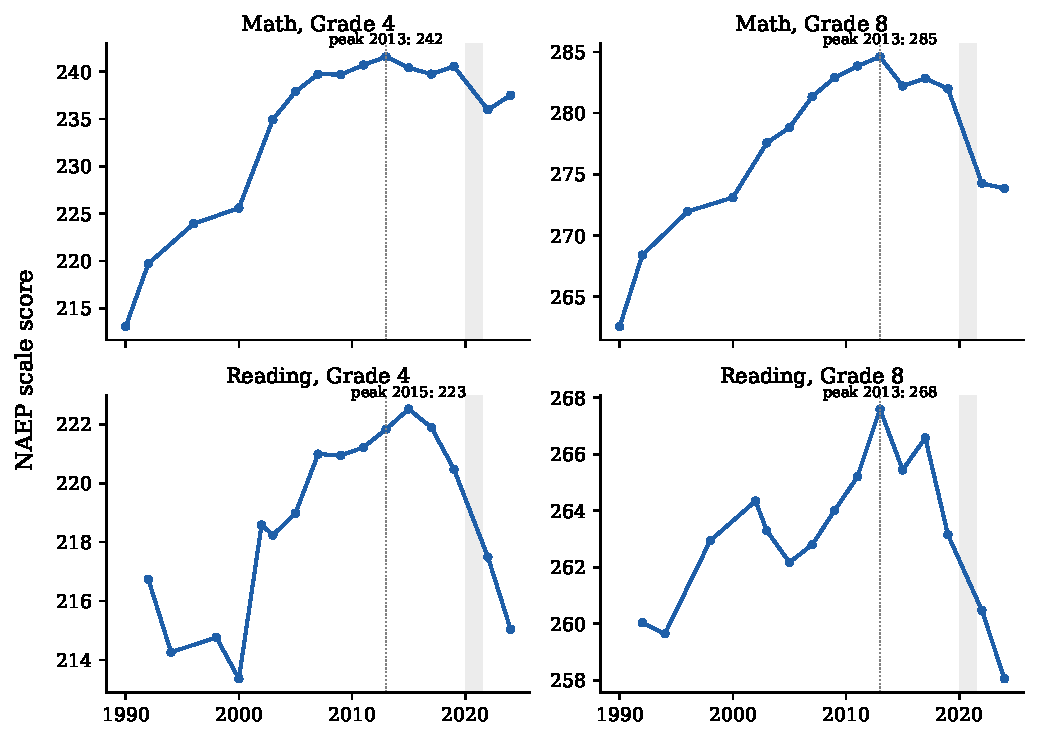
\includegraphics[width=.78\textwidth]{fig_national_trends.pdf}
\src{NAEP main assessment, national public schools. G4/G8 math and reading, 1990--2024.}
\end{frame}

\begin{frame}{Fact 2: phase one is a collapse \emph{at the bottom}}
\centering
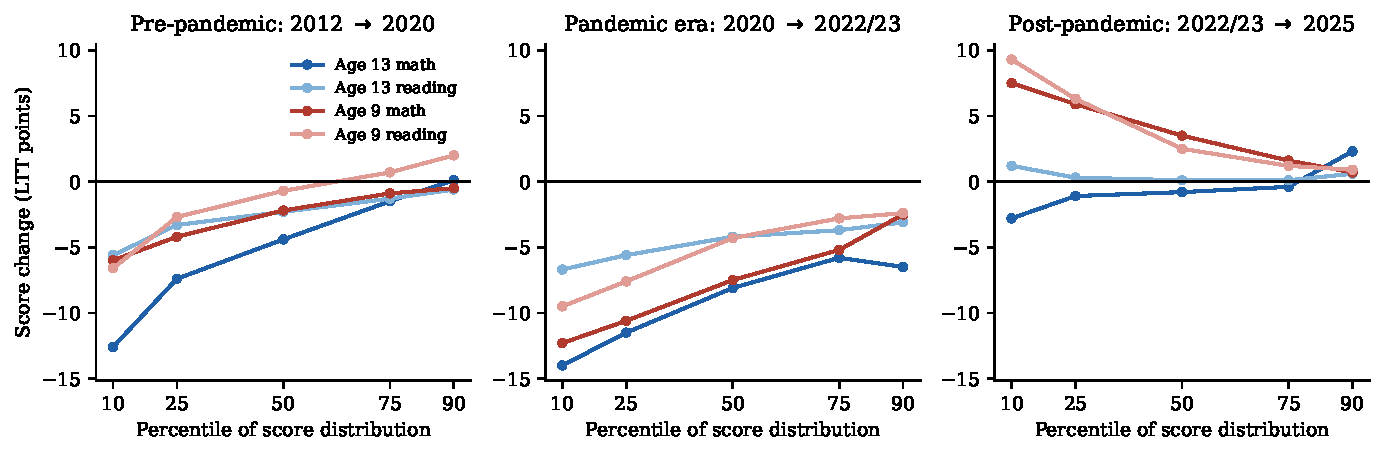
\includegraphics[width=.8\textwidth]{fig_ltt_percentiles.pdf}
\vspace{2pt}
\begin{itemize}
\item Age-13 math, 2012$\to$2020 (pre-pandemic): \red{P10 $-12.6$} vs.\ P90 $+0.1$.
\item 2022--24: the top recovers; \red{the bottom keeps falling}. G8 math 90--10 gap: 93 $\to$ 109.
\end{itemize}
\src{NAEP Long-Term Trend; main-NAEP percentile series confirm (PC:P1--P9).}
\end{frame}

\begin{frame}{Fact 3: declines occur \emph{within} every group, state, and sector}
\begin{columns}
\column{.55\textwidth}
\centering
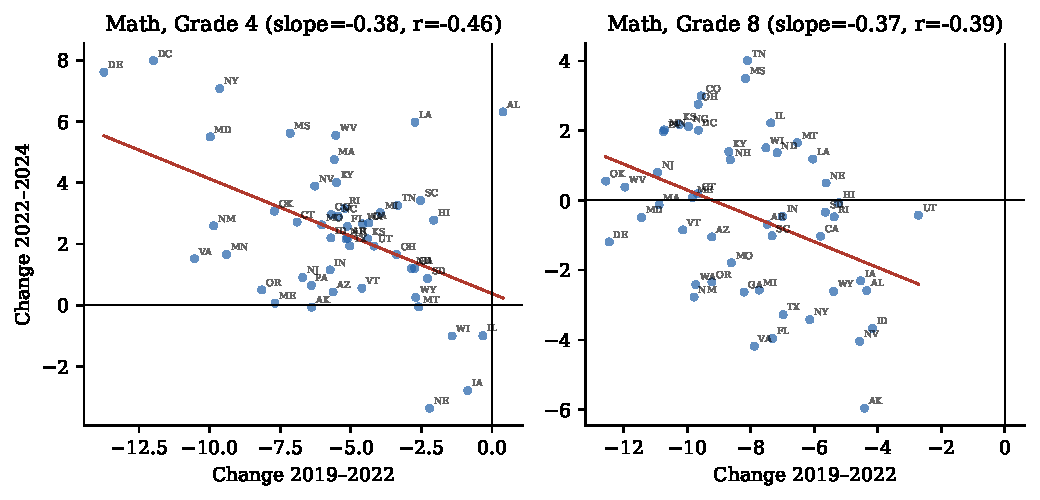
\includegraphics[width=\textwidth]{fig_states.pdf}
\column{.45\textwidth}
\begin{itemize}
\item Falling within every racial/ethnic and income group --- composition explains $\le$1--2 points.
\item Every state below its 2013 level in G8 math.
\item Same trend in Catholic schools (more below).
\end{itemize}
\end{columns}
\src{NAEP main assessment, state panels and subgroup series.}
\end{frame}

\begin{frame}{Fact 4: not just American, and not just children}
\begin{columns}
\column{.55\textwidth}
\centering
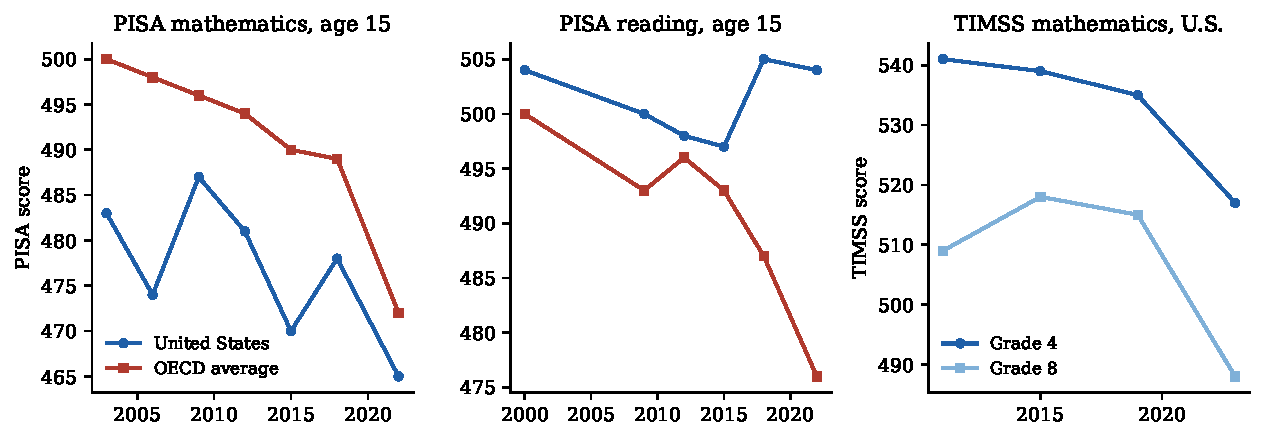
\includegraphics[width=\textwidth]{fig_intl.pdf}
\column{.45\textwidth}
\begin{itemize}
\item PISA: synchronized pre-pandemic declines across rich countries with very different school policies.
\item \textbf{Adults} (PIAAC): U.S.\ literacy \red{$-12$} 2017$\to$2023; share at/below Level 1: 19\%$\to$28\%; top stable. Declines in 19 OECD countries.
\item Same bottom-heavy signature everywhere.
\end{itemize}
\end{columns}
\src{OECD PISA 2022 Vol.~I; PIAAC Cycle 2 (caveats: 28\% U.S.\ response rate, tablet-only).}
\end{frame}

\begin{frame}{The facts any explanation must fit}
\begin{enumerate}
\item Onset $\sim$2013, well before COVID \hfill \gray{timing}
\item Concentrated at the bottom decile; top flat-to-rising pre-2020 \hfill \gray{distribution}
\item Within every demographic group and state \hfill \gray{not composition}
\item Uniform 2019--22 drop; post-2022 recovery only at the top \hfill \gray{two phases}
\item Present in Catholic schools \hfill \gray{not school policy?}
\item Synchronized internationally \hfill \gray{not U.S.\ policy}
\item Extends to adults \hfill \gray{not schooling at all?}
\item Accompanied by collapsing voluntary reading: 27\% (2012) $\to$ 14\% (2023) \hfill \gray{mechanism clue}
\end{enumerate}
\end{frame}

% ================= HYPOTHESES =================
\begin{frame}{Eight candidate explanations}
\begin{columns}[t]
\column{.5\textwidth}
\textbf{Schooling-side}
\begin{itemize}
\item[H1] Pandemic disruption
\item[H3] Retreat from NCLB accountability
\item[H4] Great-Recession funding cuts
\item[H8] Teacher quality / grade inflation
\end{itemize}
\column{.5\textwidth}
\textbf{Student/society-side}
\begin{itemize}
\item[H2] Smartphones \& digital media
\item[H5] Demographic change
\item[H6] Chronic absenteeism
\item[H7] Declining reading practice
\end{itemize}
\end{columns}
\vspace{6pt}
Strategy: derive \emph{distinct predictions} from each across timing, distribution, cohorts, sectors, geography, international scope --- then score all hypotheses against all facts.
\end{frame}

\begin{frame}{Quick kills: demographics, funding, artifacts, effort}
\begin{itemize}
\item \textbf{Demographics (H5):} declines occur within every group; compositional shift explains $\le$1--2 points of a 10+ point decline. \red{Rejected.}
\item \textbf{Funding (H4):} spending recovered after 2013 while scores kept falling; credible \$-effects are an order of magnitude too small. \red{Rejected as a primary cause.}
\item \textbf{Measurement artifacts:} exclusion flat at 1--3\% (2013--2024); participation identical in 2022 and 2024. \red{Ruled out.}
\item \textbf{Test effort:} PISA effort thermometer fell only 0.13--0.16/10 (2018$\to$2022) $\Rightarrow$ $<$5\% of the decline; same decline on consequential state tests and among adults. \red{Bounded.}
\end{itemize}
\end{frame}

% ================= SHARPER TESTS =================
\begin{frame}{Test 1 --- Cohorts: the losses accrue \emph{during adolescence}}
\begin{columns}
\column{.55\textwidth}
\centering
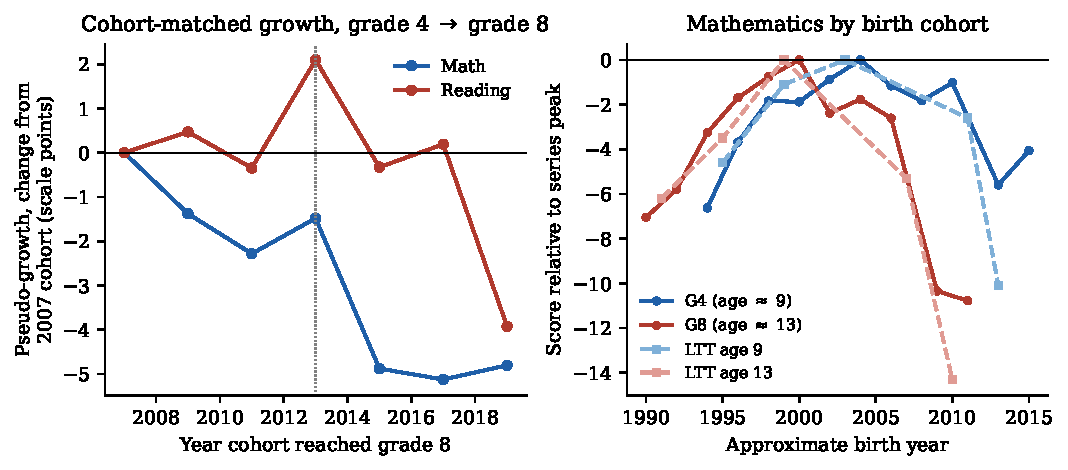
\includegraphics[width=\textwidth]{fig_cohort.pdf}
\column{.45\textwidth}
\begin{itemize}
\item Decompose every G8 change into \textbf{entry} (the cohort's G4 level) $+$ \textbf{growth} (G4$\to$G8).
\item G8 reading 2013--19: $-4.4$ = \textbf{entry $+1.6$} $-$ \textbf{growth $6.0$}.
\item Declining cohorts arrived at G4 at \emph{record} levels, then lost ground in middle school: a \red{period effect in adolescence}, not a damaged-cohort story.
\end{itemize}
\end{columns}
\src{First formal cohort/period decomposition of the decline. Blind re-derivation reproduces it to the decimal.}
\end{frame}

\begin{frame}{Test 2 --- Sectors: Catholic schools declined in step}
\begin{columns}
\column{.55\textwidth}
\centering
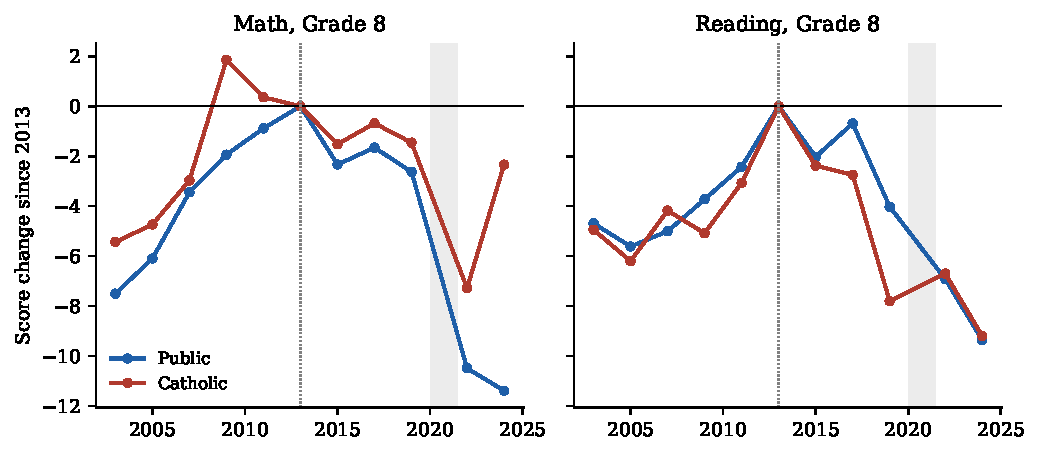
\includegraphics[width=\textwidth]{fig_pubcath.pdf}
\column{.45\textwidth}
\begin{itemize}
\item Catholic schools were \textbf{never governed} by NCLB accountability.
\item G8 reading 2013--19: Catholic \red{$-7.8$ ($z=-3.4$)} vs.\ public $-4.0$ --- at least as large.
\item Whatever drove phase one operated \emph{across} the public/private boundary.
\end{itemize}
\end{columns}
\src{NAEP SCHTYPE series; published SEs. All-private reporting ends 2013, so Catholic is the usable benchmark.}
\end{frame}

\begin{frame}{Test 3 --- Policy variation: NCLB waivers (staggered event study)}
\begin{columns}
\column{.55\textwidth}
\centering
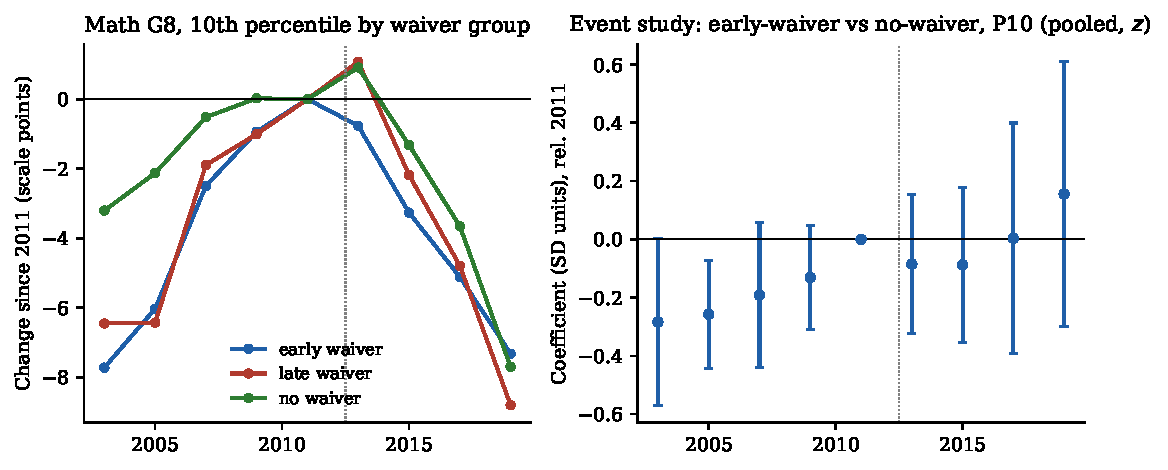
\includegraphics[width=\textwidth]{fig_waiver.pdf}
\column{.45\textwidth}
\begin{itemize}
\item States exited NCLB accountability at \textbf{different times} (2012--15); seven never did.
\item Dewey et al.\ (2026): this counterfactual has ``never been tested.''
\item Pooled DiD on state P10: $\approx$0, \textbf{permutation $p=0.46$}.
\item Informative null: \textbf{MDE$_{80}$ $\approx$ 3.2 points} --- under half the Dee--Jacob NCLB effect.
\item Caveat: joint pre-trend $p=0.08$.
\end{itemize}
\end{columns}
\src{Randomization inference, 2{,}000 permutations. Bleiberg (2020) binary/means version through 2013: also null.}
\end{frame}

\begin{frame}{Test 4 --- Common Core: never-adopters declined anyway}
\begin{columns}
\column{.55\textwidth}
\centering
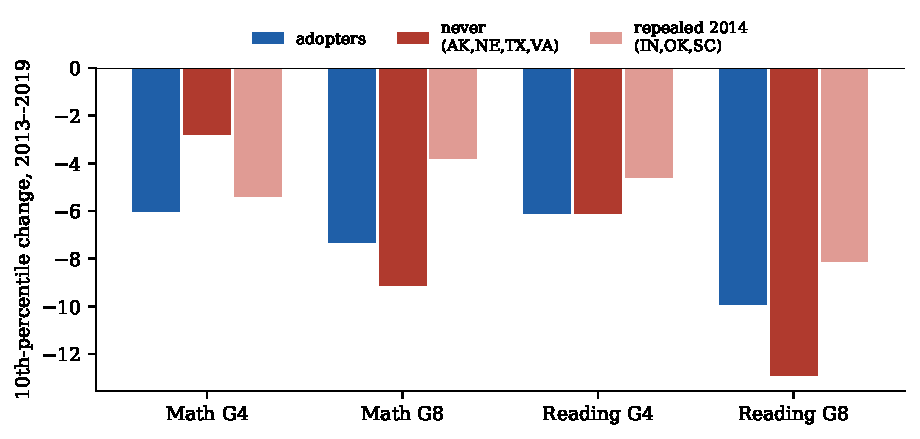
\includegraphics[width=\textwidth]{fig_commoncore.pdf}
\column{.45\textwidth}
\begin{itemize}
\item AK, NE, TX, VA never adopted; their P10 declines are \red{$\ge$ adopters'} (diff $-0.4$, $p=0.72$).
\item Minnesota (math-only non-adoption): its \emph{non-CC} subject fell \emph{less} --- wrong sign for CC harm.
\end{itemize}
\end{columns}
\src{State adoption/repeal coding; triple-difference for MN.}
\end{frame}

% ================= PHASE 2 =================
\begin{frame}{Phase two: the pandemic shock is real --- but aggregation matters}
\begin{columns}
\column{.55\textwidth}
\centering
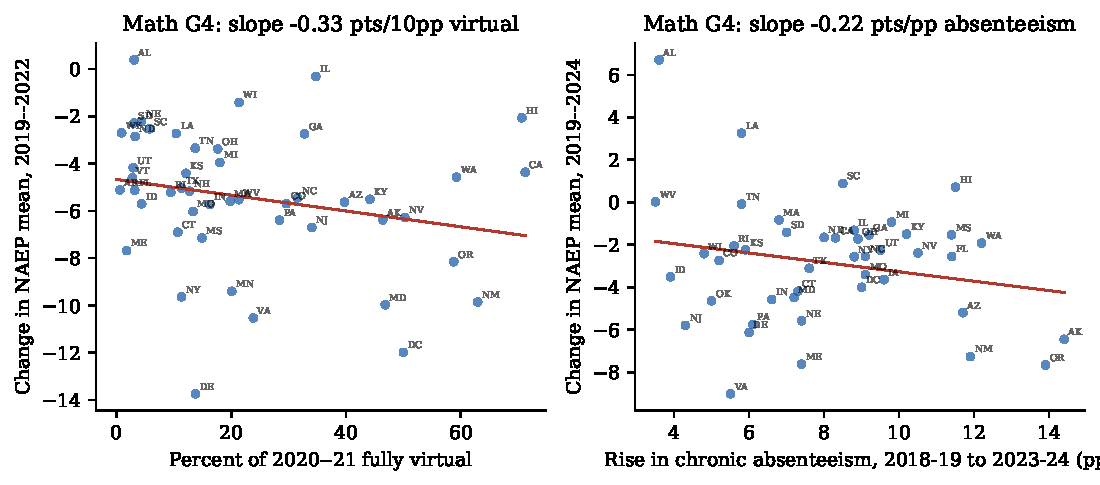
\includegraphics[width=\textwidth]{fig_doseresponse.pdf}
\column{.45\textwidth}
\begin{itemize}
\item District-level closure effects are decisive (Goldhaber et al.; Jack--Oster).
\item But \textbf{between states}, 2020-21 virtual share explains $\approx$\red{nothing} of NAEP changes ($-0.04$/10pp, $p=0.80$): state aggregation washes out district treatment variance.
\item The puzzle is not the drop --- it's the \textbf{non-recovery}.
\end{itemize}
\end{columns}
\src{CSDH schooling-mode shares $\times$ state NAEP changes; TUDA 26-district version similar (wide CIs).}
\end{frame}

\begin{frame}{The recovery brake: absenteeism --- with a pre-pandemic warning}
\begin{columns}
\column{.55\textwidth}
\centering
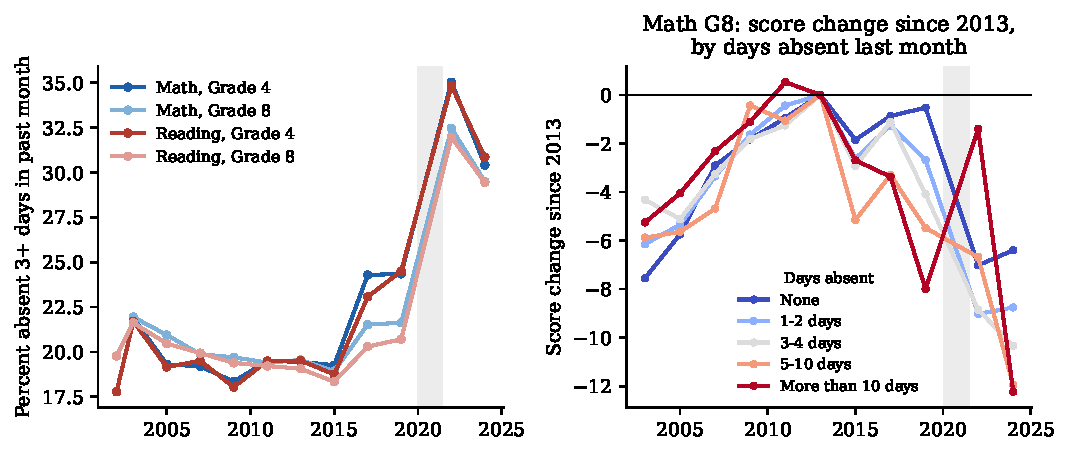
\includegraphics[width=\textwidth]{fig_absence.pdf}
\column{.45\textwidth}
\begin{itemize}
\item NAEP's own absence item: 3+ days missed last month rising \emph{before} COVID (G4: 19.5\% $\to$ 24\% by 2019), then 32--35\% in 2022, $\sim$30\% in 2024.
\item Kitagawa: the absence shift accounts for \textbf{25--42\% of 2019--24 declines} --- but only \textbf{7--19\%} of pre-pandemic G8 declines.
\item \red{Phase one was not an attendance phenomenon; phase two partly is.}
\end{itemize}
\end{columns}
\src{B018101 crosstabs; decomposition is compositional, not causal. Blind re-derivation matches exactly.}
\end{frame}

% ================= H2 EVIDENCE =================
\begin{frame}{The surviving hypothesis: digital media (H2) --- timing and mechanism}
\begin{columns}
\column{.5\textwidth}
\centering
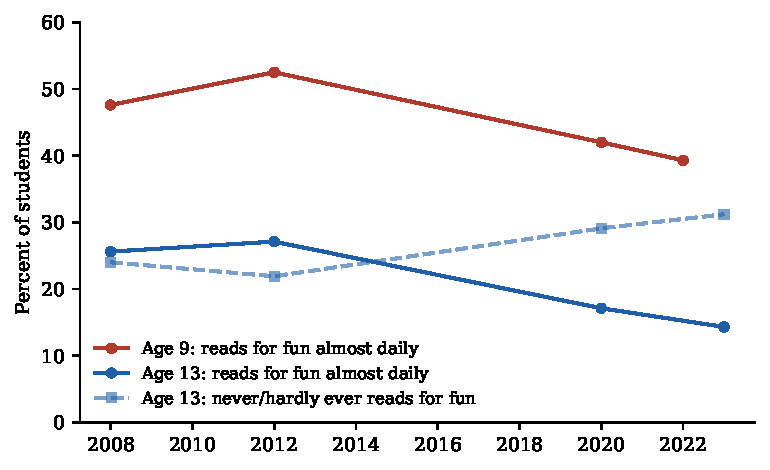
\includegraphics[width=.95\textwidth]{fig_readingfun.pdf}
\column{.5\textwidth}
\begin{itemize}
\item Teen smartphone ownership: 23\% (2011) $\to$ 73\% (2015) $\to$ 95\% (2018). The peak-and-decline sits exactly on the takeoff.
\item Reading for fun (age 13, almost daily): 27\% $\to$ 14\%, \emph{mostly pre-pandemic}.
\item H2 is the only hypothesis that natively explains the international \emph{and adult} synchrony.
\end{itemize}
\end{columns}
\src{Pew; NAEP LTT student survey (S003501).}
\end{frame}

\begin{frame}{H2 in microdata: exposure sits exactly where the damage is}
PISA 2022, 613{,}744 students; Rubin-combined PVs, school-clustered, ESCS-adjusted:
\begin{itemize}
\item Classroom device distraction (most/every lesson): \red{$-13$ (U.S.) / $-15$ (OECD)} points --- survives SES adjustment essentially intact. 5+ hrs leisure device use: $-40$.
\item Within countries, every over-engagement measure is \textbf{monotonically concentrated in the bottom score quartile} (distraction 32\% vs.\ 24\%; device anxiety 24\% vs.\ 12\%) \ldots
\item \ldots yet \textbf{nearly flat across SES quartiles} (27.9\% vs.\ 25.8\%): a low-\emph{performer} phenomenon, not a low-\emph{income} one --- matching the decline's signature in a way no compositional story does.
\item Associational, two-way causality plausible; what it establishes is that \red{the exposure profile and the damage profile coincide}.
\end{itemize}
\src{ST273Q06JA coding verified from file metadata (and independently re-derived blind). Item is rotated: U.S.\ $n\approx3{,}000$.}
\end{frame}

\begin{frame}{H2 causal corroboration from adjacent literatures}
\textbf{School phone bans (quasi-experimental):}
\begin{itemize}
\item England: $+0.064$ SD, and \red{$+0.142$ SD for low achievers, $\approx$0 for high} --- the mirror image of the decline (Beland--Murphy). Norway, Spain: similar; Florida 2023: gains by year two; Sweden's null where rules already bound.
\end{itemize}
\textbf{Fertility (new 2025--26 rollout designs, same shock):}
\begin{itemize}
\item iPhone access (AT\&T-exclusivity design) cut teen births 4.5--8\% (Myers--Hooper); 4G arrival (ruggedness IV) collapsed teen fertility, raised teen suicides (Hudson--Moscoso Boedo).
\item Effects \textbf{monotone-declining in age, null for 25+}: the critics' objection to the baby-bust claim is \red{exactly our prediction} for an adolescent learning shock.
\end{itemize}
\textbf{Cross-country:} 3G arrival $\times$ PISA, 82 countries: $-0.04$ to $-0.08$ SD (Jain--Stemper).
\end{frame}

% ================= 4G TEST =================
\begin{frame}{New test: the first within-U.S.\ mobile-rollout design on test scores}
\textbf{Design.} Archived National Broadband Map: block$\times$provider mobile coverage, 9 semiannual waves spanning the entire 2010--14 LTE rollout (validated against FCC benchmarks and Verizon's Dec-2010 launch markets). County treatment = first wave coverage $>$50\% of population. Outcomes: SEDA~5.0 county means, grades 3--8, 2009--2019 (99.9\% merge).
\vspace{4pt}
\begin{itemize}
\item Identifying variation = the \textbf{rural lag}: metro counties treated $\sim$2011--12, nonmetro 1--3 years later.
\item Estimators: Callaway--Sant'Anna event study; continuous dose (county FE + state$\times$year$\times$grade$\times$subject FE); within-county-year \textbf{adolescent-exposure gradient} across grades; permutation inference.
\end{itemize}
\src{Wyckoff (2025): direct causal smartphone$\to$achievement evidence ``lacking.'' Free data end to end; full pipeline in repo.}
\end{frame}

\begin{frame}{4G result: a precise null on the arrival-timing margin}
\begin{columns}
\column{.55\textwidth}
\centering
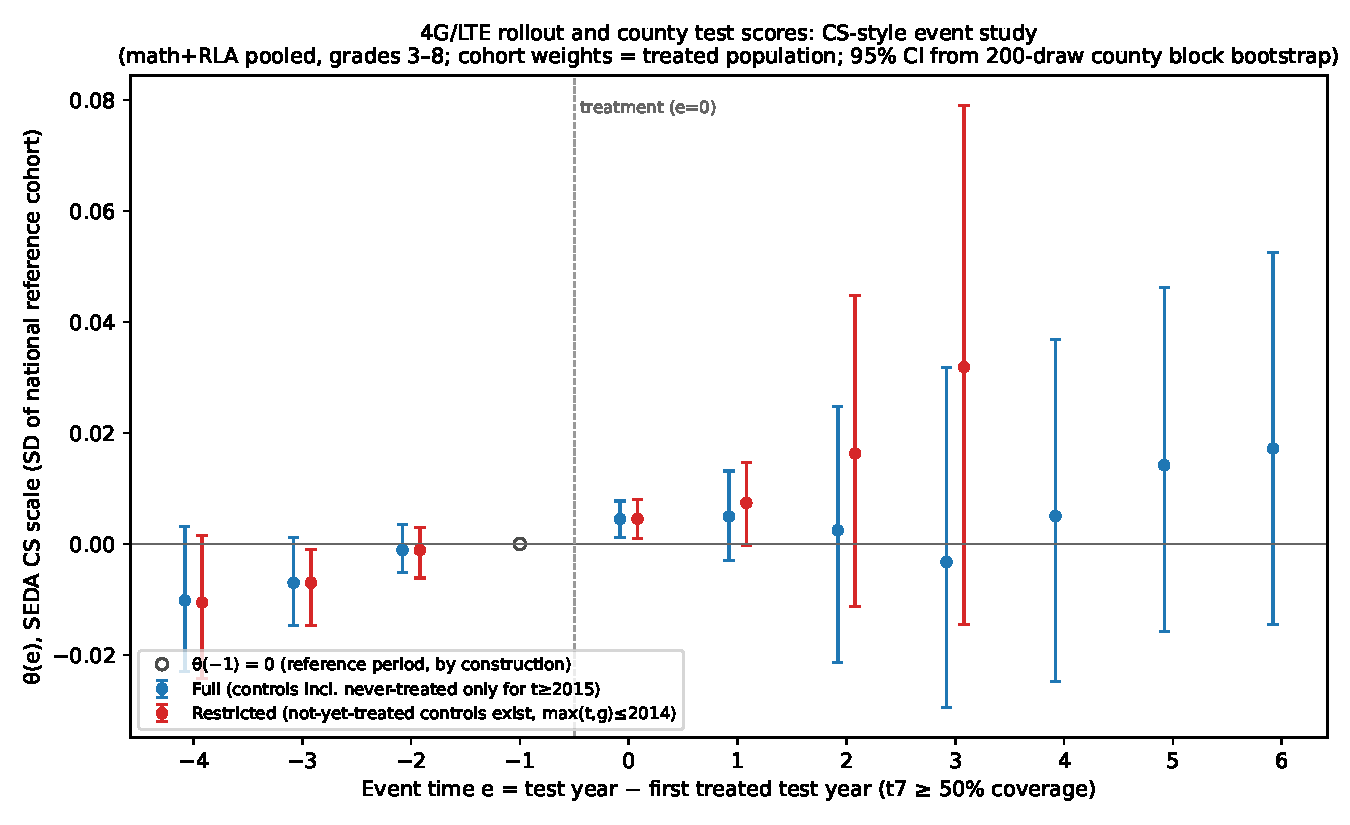
\includegraphics[width=\textwidth]{fig_4g_eventstudy.pdf}
\column{.45\textwidth}
\begin{itemize}
\item Dose: \textbf{$-0.002$ SD} (perm $p=0.66$; \textbf{MDE$_{80}=0.013$}). Gradient: $+0.011$/yr (perm $p=0.12$; MDE $0.016$).
\item 10-spec robustness grid: all $|\hat\beta|\le0.003$, signs flip. Pre-trend drift disclosed.
\item Reading: \red{the decline did not ride on local cell-tower timing.} The national, adoption-driven channel is invisible here (year FE; 3G-era adoption; controls gone by 2015).
\item Contrast: the \emph{same} variation moves teen fertility --- not test scores.
\end{itemize}
\end{columns}
\end{frame}

% ================= SYNTHESIS =================
\begin{frame}{Synthesis: a dual-criterion test}
Borrowed from the fertility-puzzle debate (Kearney--Levine; Evans): a candidate cause must clear \textbf{two bars at once}:
\begin{enumerate}
\item \textbf{Synchrony:} explain the same decline across countries with disparate school systems --- and among adults.
\item \textbf{Signature:} explain bottom-of-distribution concentration, adolescent-period timing, sector neutrality.
\end{enumerate}
\vspace{4pt}
\begin{itemize}
\item Every school-policy explanation \red{fails bar 1 by construction}.
\item The pandemic \red{fails bar 2} for phase one (it arrived six years late).
\item \textbf{Digital media is the only candidate examined that clears both.} Accountability retreat retains a marginal supporting role (G4 public bottom decile); absenteeism owns the phase-two non-recovery.
\end{itemize}
\end{frame}

\begin{frame}{Scorecard}
\centering\scriptsize
\setlength{\tabcolsep}{4pt}
\begin{tabular}{lcccccc}
\toprule
 & Timing & Bottom-heavy & COVID drop & No recovery & Within-grp & Int'l \\
\midrule
H1 Pandemic            & $\times$ & $\sim$ & \checkmark & $\sim$ & \checkmark & $\sim$ \\
\textbf{H2 Digital media} & \checkmark & $\sim$ & $\times$ & \checkmark & \checkmark & \checkmark \\
H3 Accountability      & \checkmark & \checkmark & $\times$ & $\sim$ & \checkmark & $\times$ \\
H4 Funding cuts        & $\sim$ & $\times$ & $\times$ & $\times$ & $\sim$ & $\times$ \\
H5 Demographics        & $\times$ & $\times$ & $\times$ & $\times$ & $\times$ & $\times$ \\
\textbf{H6 Absenteeism} & $\times$ & \checkmark & \checkmark & \checkmark & \checkmark & $\sim$ \\
H7 Reading practice    & \checkmark & $\sim$ & $\times$ & \checkmark & \checkmark & \checkmark \\
H8 Teachers/inflation  & $\sim$ & $\sim$ & $\times$ & $\sim$ & $\sim$ & $\times$ \\
\bottomrule
\end{tabular}
\vspace{4pt}

{\small Two-phase accounting: phase one $\approx$ 20--45\% of the total 2013--24 decline; pandemic window 30--70\%; post-2022 the rest. \red{Full COVID recovery would still leave the U.S.\ far below 2013.}}
\end{frame}

% ================= NEXT / CONCLUSION =================
\begin{frame}{What would settle it: a pre-registered test arriving in 2027}
\begin{itemize}
\item $\sim$30 states adopted school phone bans between 2023--24 and 2025--26, with staggered timing and varying bindingness (bell-to-bell vs.\ instructional-time).
\item \textbf{Pre-registered design} (frozen before data exist): exposure groups from 50-state statute coding; NAEP 2026 state percentiles; same permutation machinery as the waiver test.
\item Predictions on record: gains at P10/P25, larger under bell-to-bell bans; top decile $\approx$ flat.
\item This is the waiver test's logic pointed at the leading hypothesis --- with $\sim$4$\times$ the treated states.
\end{itemize}
\vspace{4pt}
Also on the docket: restricted-use NAEP microdata; PISA 2012$\to$2022 ICT panel; SEDA/adoption-margin designs.
\end{frame}

\begin{frame}{Conclusion}
\begin{enumerate}
\item The decline is real, large, verifiable --- and \textbf{older than COVID}.
\item It is a crisis of the \textbf{struggling student}: bottom-decile collapse, record gaps.
\item Direct tests reject the school-policy suspects; the evidence triangulates to \textbf{digital media} for phase one and \textbf{absenteeism-sustained pandemic damage} for phase two.
\item Policy implications: treat attendance as the front line; take \emph{binding} phone restrictions seriously (2026 will tell); target the bottom of the distribution; and do not mistake ``back to 2019'' for recovery --- \red{2019 was already pointing down}.
\end{enumerate}
\vfill
\gray{\small Paper, data, code, claims audit, and pre-registration: github.com/brendanbartanen-svg/naep-achievement-decline}
\end{frame}

% ================= APPENDIX =================
\appendix
\begin{frame}{Appendix: verification layer}
\begin{itemize}
\item \textbf{Claims audit:} 41 load-bearing claims, each typed (citation/pulled/computed) with a $<$5-minute verification path; 62-assertion test suite runs clean.
\item \textbf{Blind clean-room replications} (independent agents, no access to analysis code, fresh API/microdata pulls) --- \textbf{5/5 reproduce}, no pipeline errors:
  \begin{itemize}
  \item Cohort decomposition exact ($-4.45 = +1.57 - 6.02$); PISA distraction exact U.S.\ ($-13.25$), item coding independently recovered from file metadata; Kitagawa data to the decimal; Catholic-sector changes exact (official NAEP tests agree); waiver null + MDE confirmed, point estimate spec-dependent ($\approx$0).
  \end{itemize}
\item \textbf{External anchors:} waiver null $\leftrightarrow$ Bleiberg (2020); state-aggregation null $\leftrightarrow$ Goldhaber/Jack--Oster; sector pattern $\leftrightarrow$ Malkus/Petrilli; PISA gaps $\leftrightarrow$ OECD published bivariates; 4G panel $\leftrightarrow$ FCC benchmarks + Verizon launch markets.
\item \textbf{Human verification:} all four hand-coded policy datasets spot-checked against primary documents; five headline numbers re-pulled manually from the NAEP Data Explorer; Synthesis section adversarially reviewed by an independent colleague.
\item Full record: report \S Verification; \texttt{evidence/claims\_audit.md}; \texttt{verification/cleanroom/COMPARISON.md}.
\end{itemize}
\end{frame}

\begin{frame}{Appendix: 4G robustness grid}
\centering\small
\begin{tabular}{lcc}
\toprule
Specification & Coef.\ (SD) & $p$ (cluster) \\
\midrule
Dose, t7 (primary) & $-0.0022$ & .57 \\
Binary first\_t7\_50 & $-0.0017$ & .58 \\
Binary first\_t6\_50 & $-0.0030$ & .35 \\
Binary first\_t7\_25 & $-0.0022$ & .52 \\
Binary first\_t7\_75 & $-0.0029$ & .28 \\
Binary t6\_50, Verizon-only & $-0.0010$ & .81 \\
Dose, drop artifact states & $+0.0015$ & .64 \\
Binary t7\_50, drop artifact states & $+0.0013$ & .63 \\
Dose, unweighted & $+0.0004$ & .92 \\
Binary t7\_50, unweighted & $+0.0007$ & .81 \\
\bottomrule
\end{tabular}
\vspace{4pt}

{\small County FE + state$\times$year$\times$grade$\times$subject FE; SEs clustered by state; permutation inference within state.}
\end{frame}

\begin{frame}{Appendix: avenues examined and set aside}
\begin{itemize}
\item \textbf{Opioid exposure:} state correlations null/inconsistent --- tested and cut.
\item \textbf{Cannabis legalization, discipline reform:} no clean variation --- documented set-asides.
\item \textbf{Cross-country smartphone-adoption timing:} data quality insufficient.
\item \textbf{PISA leisure-hours items (ST326/ST322):} not administered in the U.S.; the IC171 fallback is an access artifact in a 95\%-saturated population --- cut.
\item \textbf{TUDA district dose-response:} weak gradient, wide CIs --- limitation, not contradiction, of district-level closure findings.
\end{itemize}
\end{frame}

\end{document}
